\section{Datenstrukturen}

\begin{frame}{Hashtable}
 	\begin{block}{Hashing}
	 	\begin{itemize}
	 		\item (Schnelles) Finden durch Unordnung
	 		\item \enquote{to hash} = zerhacken
			\pause
	 		\item Trick: Hashfunktionen bilden (komplexe) Objekte (durcheinander) auf einfache Zahlen (Hashwerte) ab
	 		\item Hashwerte dienen als Indizes in der Hashtabelle
	 		\item Folge: (Fast) direkte Abbildung Schlüsselobjekt $\rightarrow$ Element
	 	\end{itemize}
 	\end{block}
 	
 	\pause
 	
 	\begin{center}
		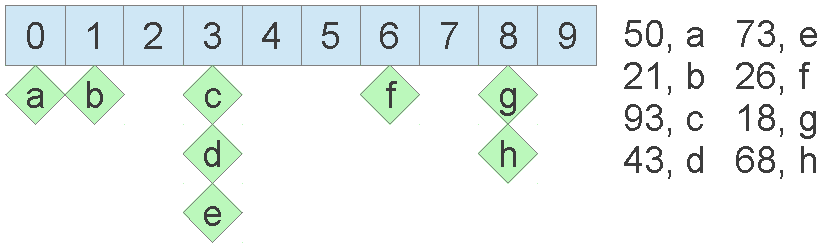
\includegraphics[width=0.95\linewidth]{images/hashmap.pdf}
	\end{center}
\end{frame}

\begin{frame}{Hashtables in C++}
 	\begin{itemize}
 		\item boost::intrusive::hashtable
 		\item SGI-Extensions zur STL
 		\item C++11: \texttt{unordered\_(multi)map} und darauf basierend: \texttt{unordered\_(multi)set}
 	\end{itemize}
 	
 	\pause
 	
 	\begin{block}{\texttt{std::unordered\_map}}
	 	\begin{itemize}
	 		\item \texttt{insert(pair<key, value>)}
	 		\item \texttt{find(key)}
	 		\item \texttt{erase(key)}
	 	\end{itemize}
	 	\pause
	 	Alles (amortisiert) in $\mathcal{O}(1)$
 	\end{block}
\end{frame}

